\chapter{Model Wienera}
Istota modelu Wienera jest dokładnie taka sama jak w przypadku modelu Hammersteina z tym, że nieliniową statykę poprzedzono liniową dynamika - odwrotnie niż jak to było w przypadku omówionego modelu.

\begin{figure}[h!]
\centering
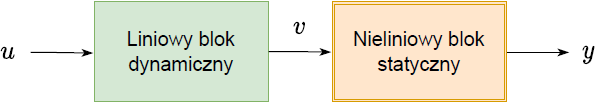
\includegraphics[width=\textwidth]{pictures/wien_model}
\caption{Reprezentacja graficzna modelu Wienera.}
\end{figure}

Sygnał wejściowy trafia na liniowy blok dynamiczny, gdzie jest przekonwertowany na sygnał $v = f(u)$, który trafia na nieliniową statykę, której wyjściem jest sygnał $y$. W przypadku dynamiki skorzystano z wyznaczonego wcześniej modelu dynamicznego (\ref{diff_eq}), natomiast zmianie uległa charakterystyka statyczna.

\section{Następniki liniowe}
W przypadku modelu Wienera aproksymacja charakterystyki statycznej przysporzyła więcej problemów niżeli w przypadku modelu Hammersteina. Przyjęty przedział rozmywania zmiennej $v \in [-25;25]$ podzielono na pięć zbiorów.

\begin{figure}[h!]
\centering
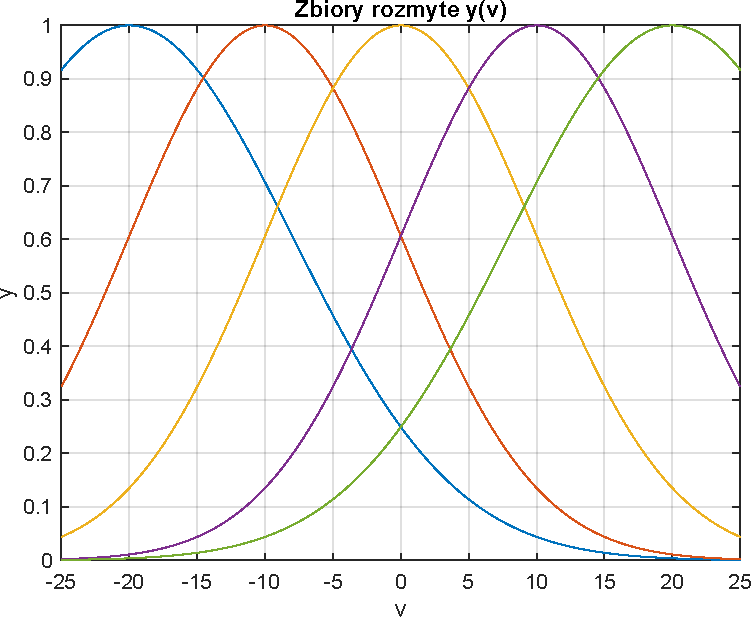
\includegraphics[width=0.6\textwidth]{pictures/fuzzy_set_wien}
\caption{Zbiory rozmyte - następniki liniowe.}
\end{figure}

\newpage

\noindent Dzięki zastosowanemu podziałowi udało się otrzymać następującą aproksymację charakterystyki statycznej.

\begin{figure}[h!]
\centering
\subfloat[Zbiór uczący.]{
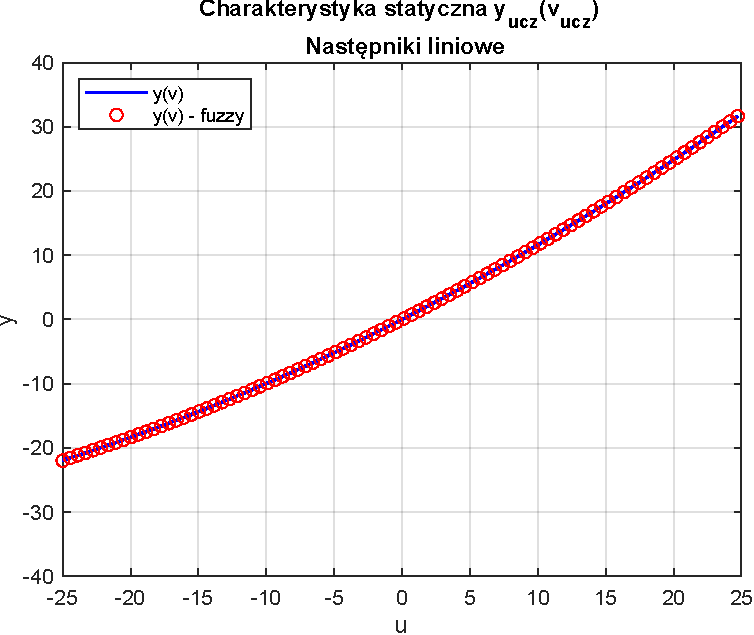
\includegraphics[width=0.45\textwidth]{pictures/static_char_wien_lin_ucz}}
\hfill
\subfloat[Zbiór weryfikujący]{
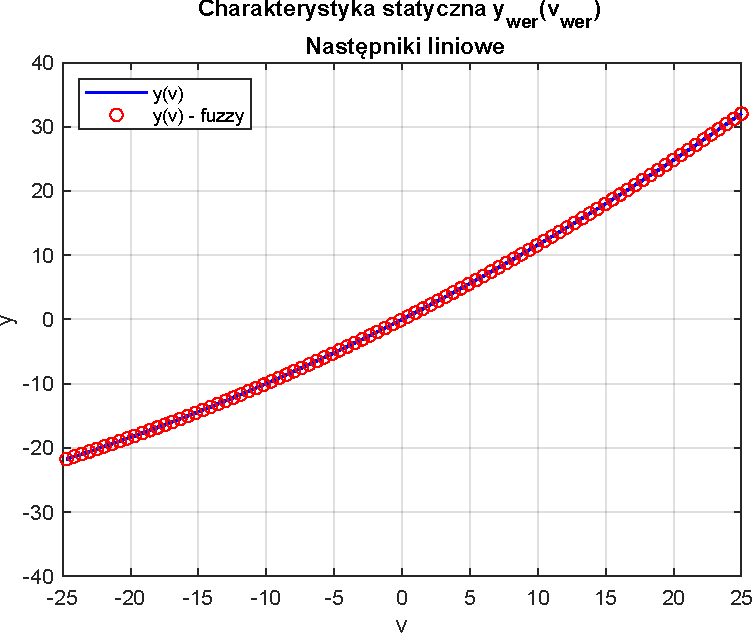
\includegraphics[width=0.45\textwidth]{pictures/static_char_wien_lin_wer}}
\caption{Aproksymacja charakterystyki statycznej przez model rozmyty - następniki liniowe.}
\end{figure}

Następniki liniowe reguł przybrały postać zaprezentowaną w \ref{nastepniki_lin}. Ponownie pierwsze przybliżenie zostało wyznaczone w za pomocą funkcji MATLAB, tym razem jednak niezbędne okazało się ręczne dostrajanie otrzymanych współczynników. Do problemu zdecydowano podejść w następujący sposób - starano się minimalizować błąd zbioru uczącego, następnie analizowano zachowanie modelu w przypadku zbiory weryfikującego. Wygenerowano kilka sekwencji sygnału sterującego i porównano zachowanie modelu dynamicznego i modelu Wienera.

\newpage

%%%%%%%%%%%%%%%%%%%%%% PIERWSZA SEKWENCJA %%%%%%%%%%%%%%%%%%%%%%
\begin{figure}[h!]

\begin{center}
\Large \textbf{I sekwencja} \\
\vspace{0.5cm}
\Large \textbf{Model dynamiczny}
\end{center}

\centering
\subfloat[Zbiór uczący.]{
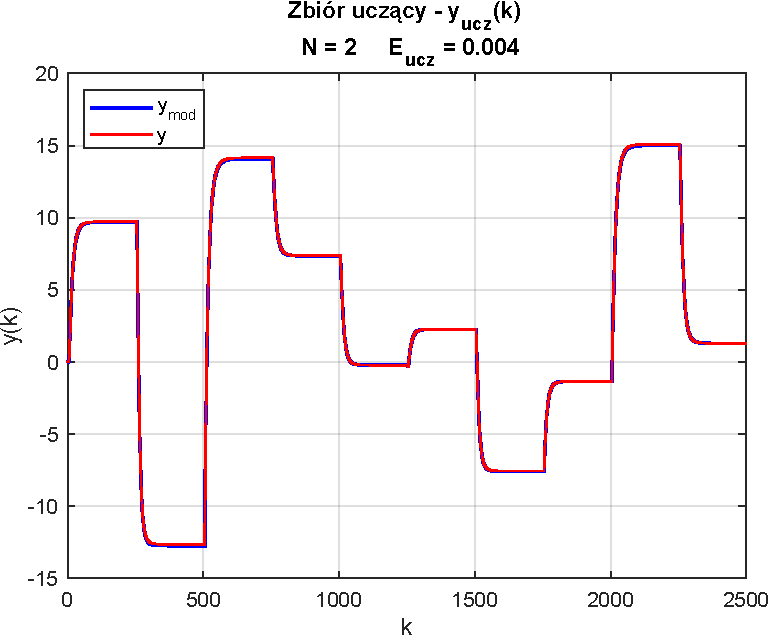
\includegraphics[width=0.45\textwidth]{pictures/arx_ucz_11}}
\hfill
\subfloat[Zbiór weryfikujący]{
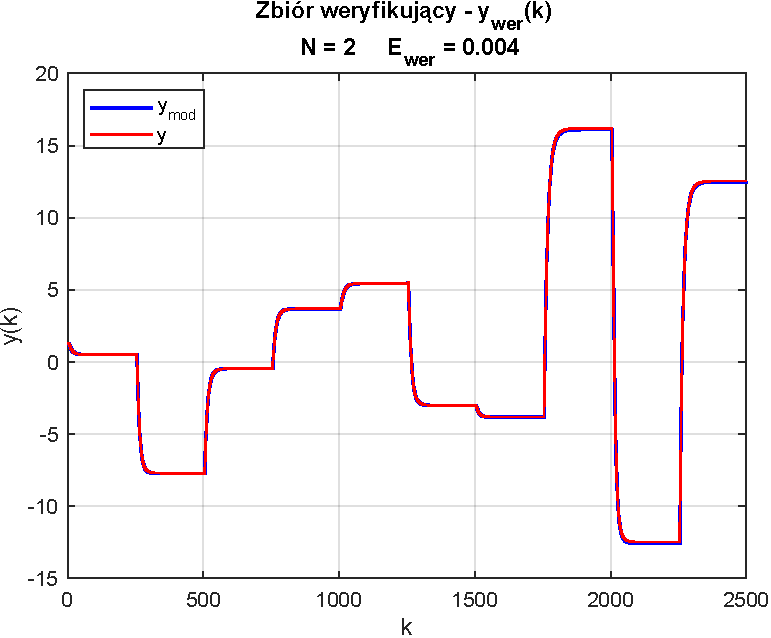
\includegraphics[width=0.45\textwidth]{pictures/arx_wer_11}}

\begin{center}
\Large \textbf{Model Wienera}
\end{center}

\subfloat[Zbiór uczący.]{
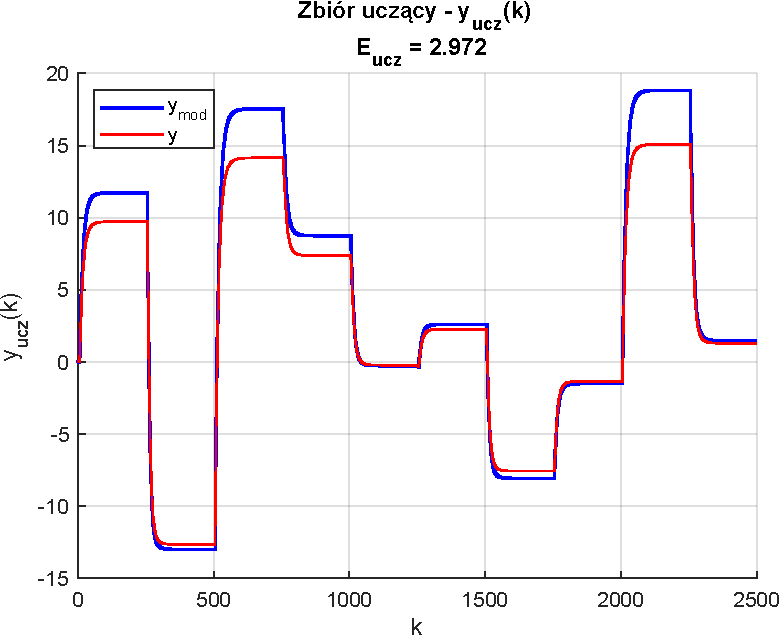
\includegraphics[width=0.45\textwidth]{pictures/arx_wien_ucz_11}}
\hfill
\subfloat[Zbiór weryfikujący]{
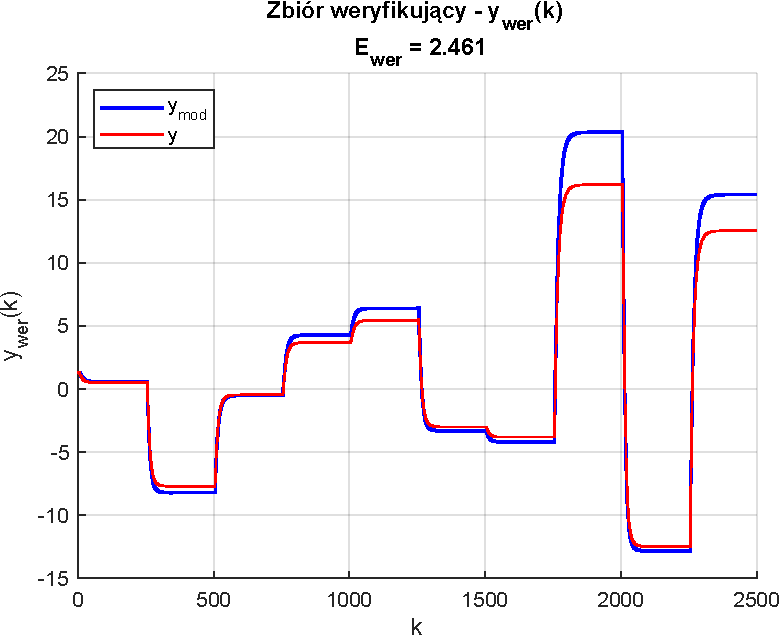
\includegraphics[width=0.45\textwidth]{pictures/arx_wien_wer_11}}
\caption{Porównanie przebiegu sygnału wyjściowego modelu dynamicznego i modelu Wienera w trybie bez rekurencji.}
\end{figure}

Jak widać na powyższych rysunkach dokładność osiągnięta przez model Wienera w trybie ARX jest nieakceptowalna - postanowiono ręcznie dostroić model. Dokonano tego tylko poprzez zmianę wartości współczynników lokalnych modeli systemu rozmytego. Uzyskane rezultaty zaprezentowano na rys. \ref{wien_arx}.

\newpage

\begin{figure}[h!]
\centering
\subfloat[Zbiór uczący.]{
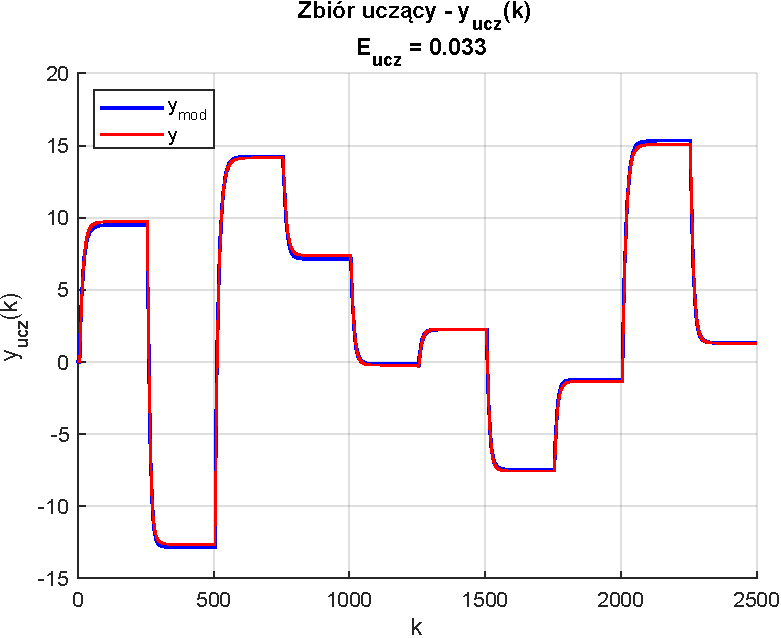
\includegraphics[width=0.7\textwidth]{pictures/arx_wien_ucz_12}}
\vfill
\subfloat[Zbiór weryfikujący]{
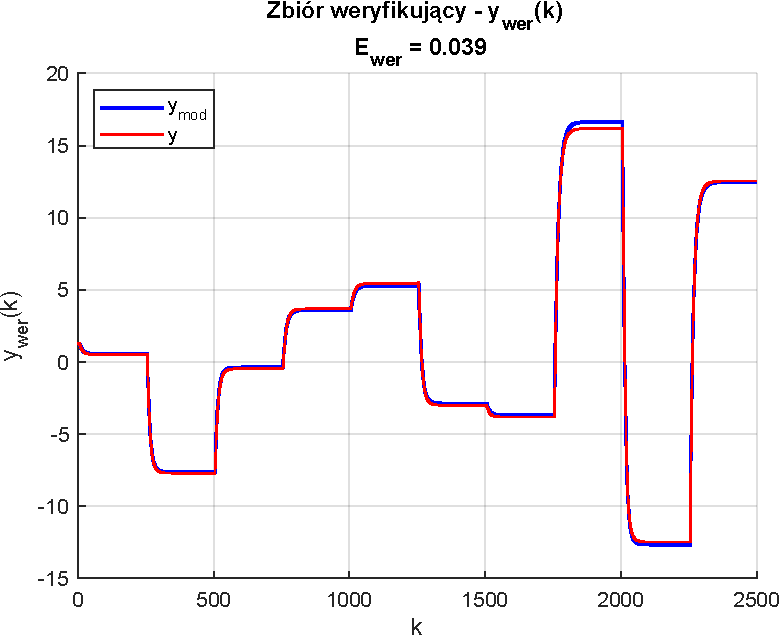
\includegraphics[width=0.7\textwidth]{pictures/arx_wien_wer_12}}
\caption{Przebiegu sygnału wyjściowego modelu Wienera w trybie bez rekurencji po dostrojeniu współczynników następników.}
\label{wien_arx}
\end{figure}

Model Wienera po ręcznym strojeniu osiągnął próg akceptowalności w kontekście kryterium jakości - $E = \num{0.1}$. Analogiczne podejście zastosowano w przypadku testowania modelu w trybie rekurencyjnym.

\newpage

\begin{figure}[h!]

\begin{center}
\Large \textbf{I sekwencja} \\
\vspace{0.5cm}
\Large \textbf{Model dynamiczny}
\end{center}

\centering
\subfloat[Zbiór uczący.]{
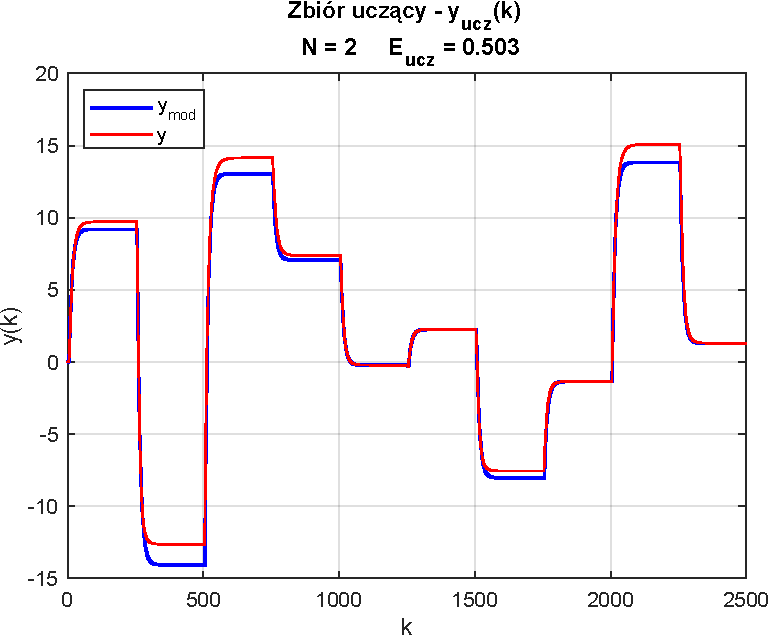
\includegraphics[width=0.45\textwidth]{pictures/oe_ucz_11}}
\hfill
\subfloat[Zbiór weryfikujący]{
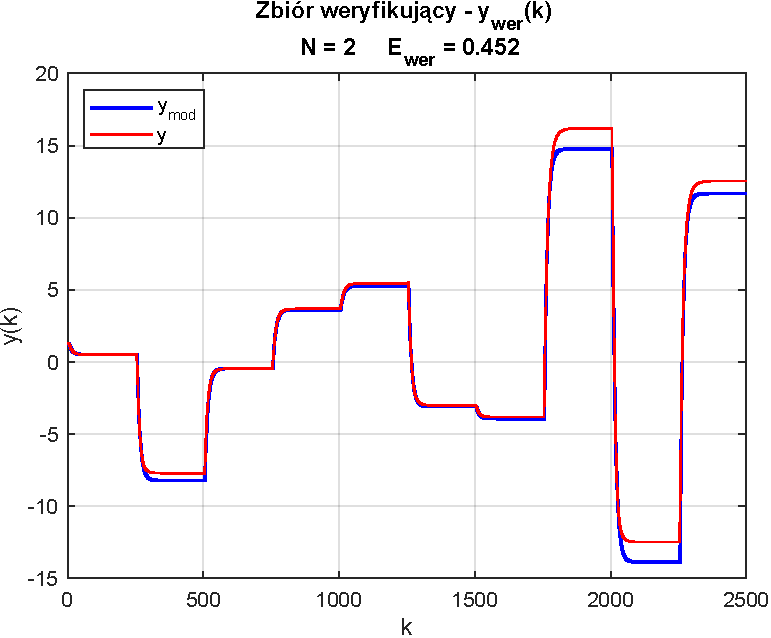
\includegraphics[width=0.45\textwidth]{pictures/oe_wer_11}}

\begin{center}
\Large \textbf{Model Wienera}
\end{center}

\subfloat[Zbiór uczący.]{
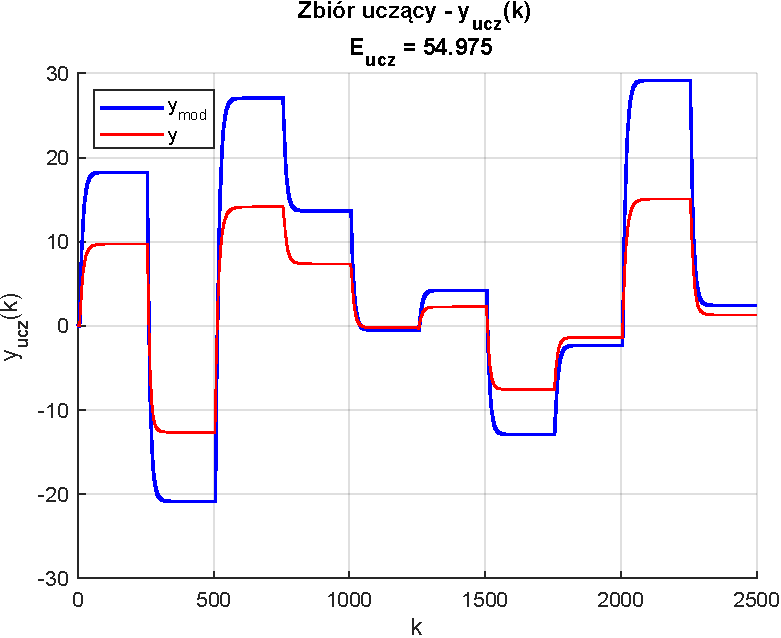
\includegraphics[width=0.45\textwidth]{pictures/oe_wien_ucz_11}}
\hfill
\subfloat[Zbiór weryfikujący]{
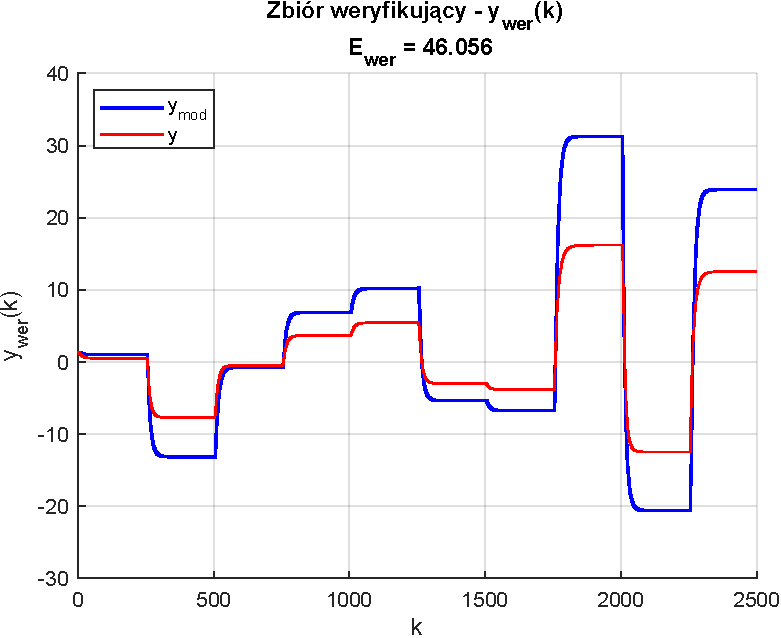
\includegraphics[width=0.45\textwidth]{pictures/oe_wien_wer_11}}
\caption{Porównanie przebiegu sygnału wyjściowego modelu dynamicznego i modelu Wienera w trybie rekurencyjnym.}
\end{figure}

Model Wienera w trybie rekurencyjnym osiągnął bardzo duże wartości błędów. Natomiast postanowiono przyjąć inną strategię dostrajania, widać bowiem, że przemnożenie wyjścia modelu przez pewną stałą dałoby już zadowalający rezultat. Konieczne okazało się również dostrojenie wartości poszczególnych współczynników modeli lokalnych systemu rozmytego, aby osiągnąć zakładaną dokładność. Efekt przedstawiono na rys. \ref{wien_oe}.

\newpage

\begin{figure}[h!]
\centering
\subfloat[Zbiór uczący.]{
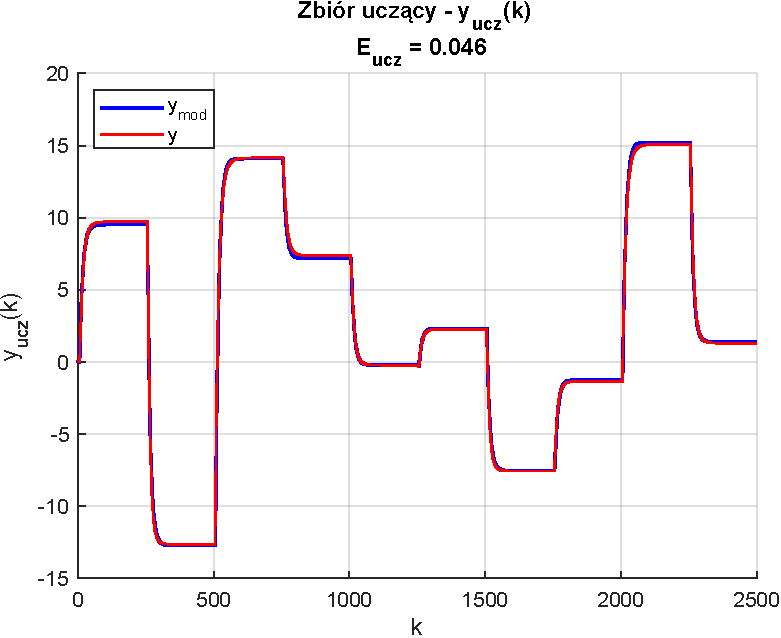
\includegraphics[width=0.7\textwidth]{pictures/oe_wien_ucz_12}}
\vfill
\subfloat[Zbiór weryfikujący]{
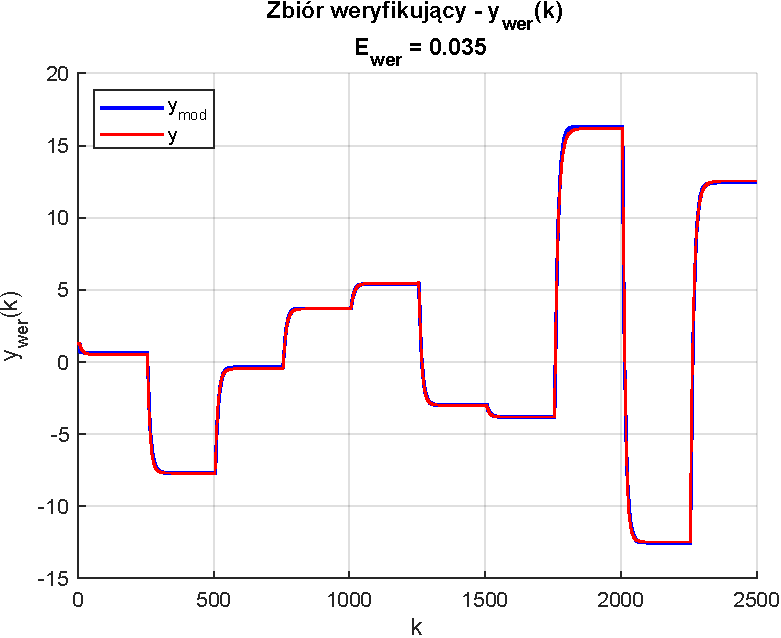
\includegraphics[width=0.7\textwidth]{pictures/oe_wien_wer_12}}
\caption{Przebiegu sygnału wyjściowego modelu Wienera w trybie rekurencyjnym po dostrojeniu współczynników następników.}
\label{wien_oe}
\end{figure}

Jak pokazują powyższe ilustracje osiągnięto satysfakcjonującą dokładność, zbliżoną do tych uzyskanych podczas symulacji modelu Hammersteina (w niektórych przypadkach nawet lepszą). Dostrojony model poddano testom, generując kolejne dwie sekwencje sygnału sterującego.

%%%%%%%%%%%%%%%%%%%%%% DRUGA SEKWENCJA %%%%%%%%%%%%%%%%%%%%%%

\begin{figure}[p!]

\begin{center}
\Large \textbf{II sekwencja} \\
\vspace{0.5cm}
\Large \textbf{Model dynamiczny}
\end{center}

\centering
\subfloat[Zbiór uczący.]{
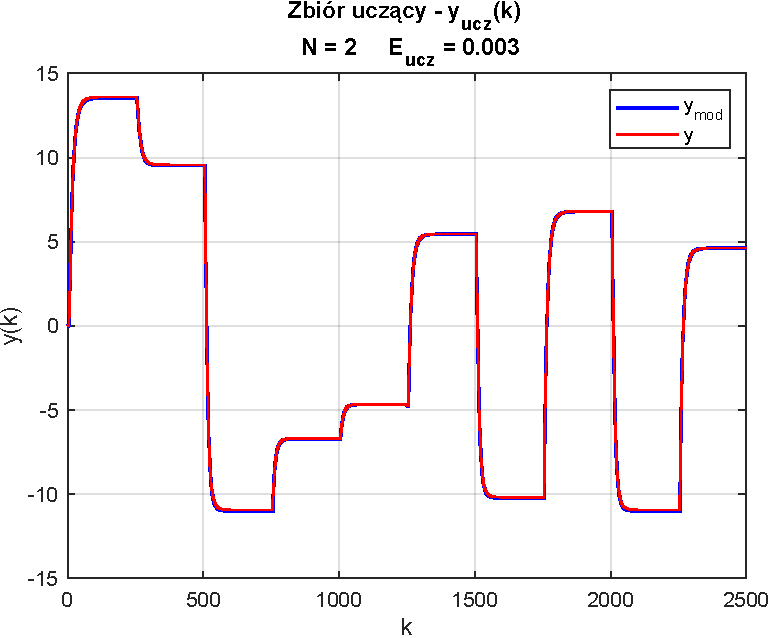
\includegraphics[width=0.45\textwidth]{pictures/arx_ucz_22}}
\hfill
\subfloat[Zbiór weryfikujący.]{
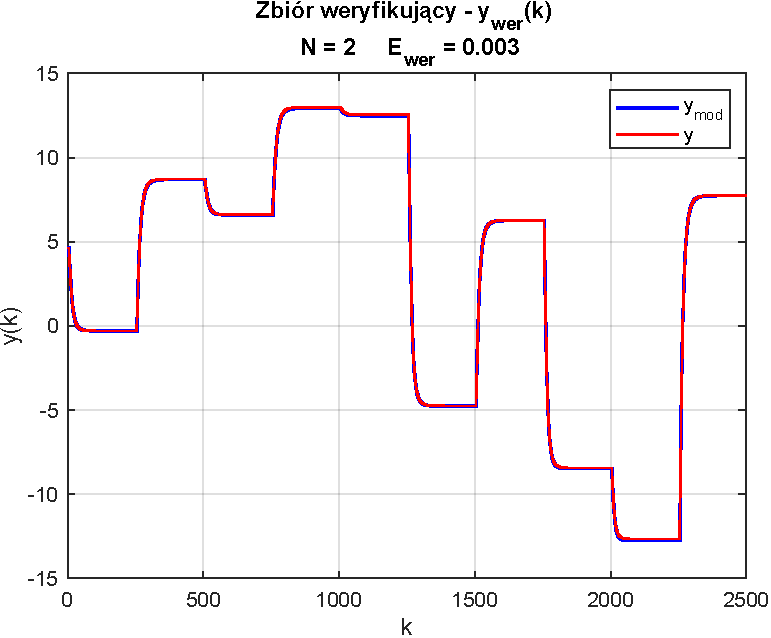
\includegraphics[width=0.45\textwidth]{pictures/arx_wer_22}}

\begin{center}
\Large \textbf{Model Wienera}
\end{center}

\subfloat[Zbiór uczący.]{
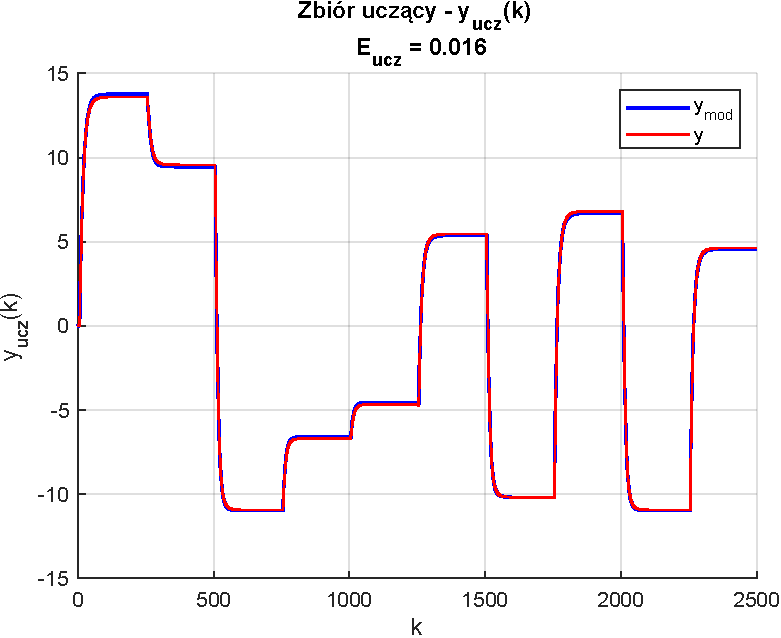
\includegraphics[width=0.45\textwidth]{pictures/arx_wien_ucz_22}}
\hfill
\subfloat[Zbiór weryfikujący.]{
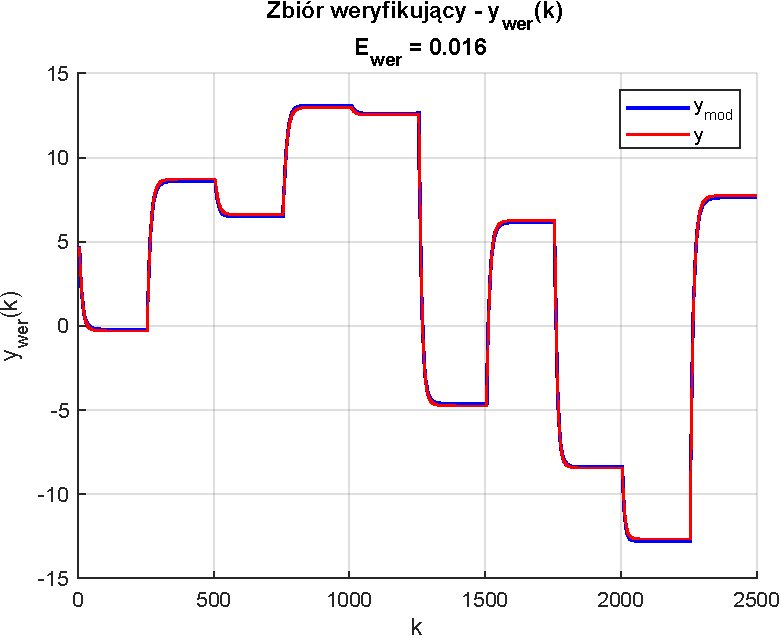
\includegraphics[width=0.45\textwidth]{pictures/arx_wien_wer_22}}
\caption{Porównanie przebiegu sygnału wyjściowego modelu dynamicznego i modelu Wienera w trybie bez rekurencji.}
\end{figure}

\begin{figure}[p!]

\begin{center}
\Large \textbf{II sekwencja} \\
\vspace{0.5cm}
\Large \textbf{Model dynamiczny}
\end{center}

\centering
\subfloat[Zbiór uczący.]{
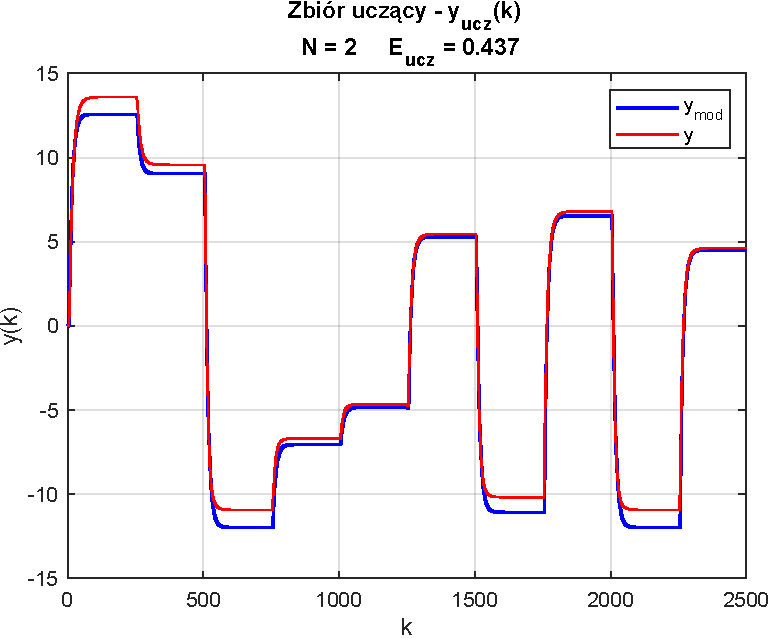
\includegraphics[width=0.45\textwidth]{pictures/oe_ucz_22}}
\hfill
\subfloat[Zbiór weryfikujący.]{
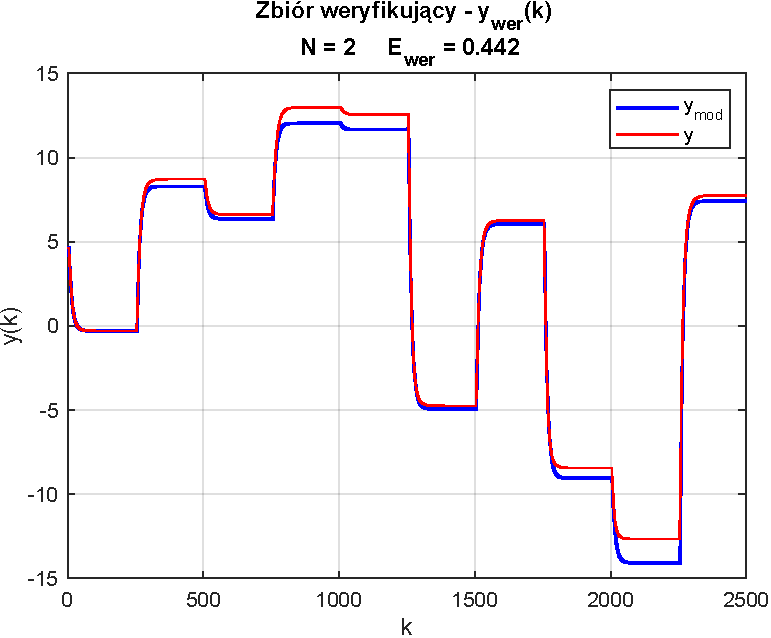
\includegraphics[width=0.45\textwidth]{pictures/oe_wer_22}}

\begin{center}
\Large \textbf{Model Wienera}
\end{center}

\subfloat[Zbiór uczący.]{
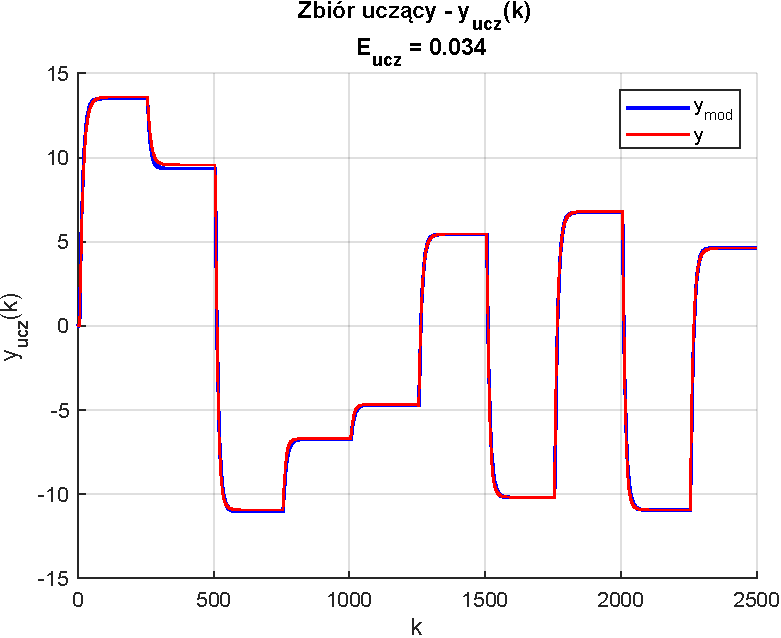
\includegraphics[width=0.45\textwidth]{pictures/oe_wien_ucz_22}}
\hfill
\subfloat[Zbiór weryfikujący.]{
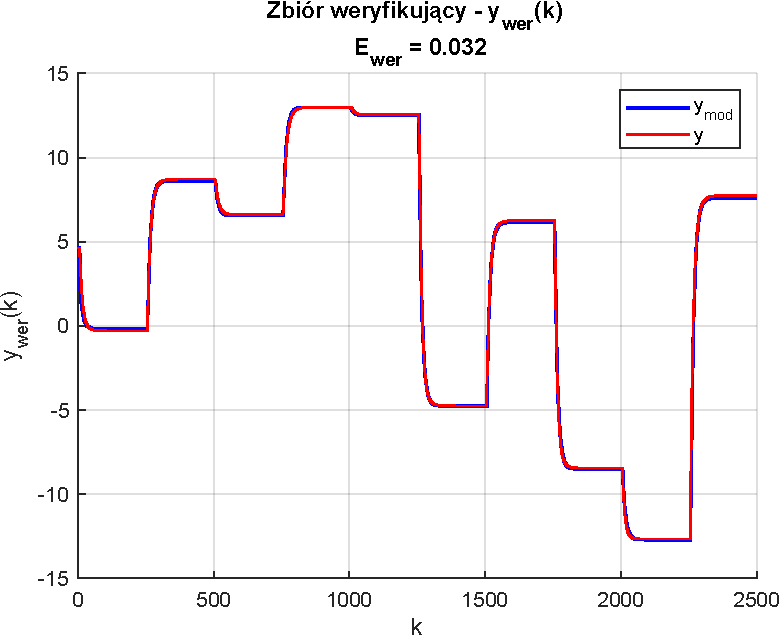
\includegraphics[width=0.45\textwidth]{pictures/oe_wien_wer_22}}
\caption{Porównanie przebiegu sygnału wyjściowego modelu dynamicznego i modelu Wienera w trybie rekurencyjnym.}
\end{figure}

%%%%%%%%%%%%%%%%%%%%%% TRZECIA SEKWENCJA %%%%%%%%%%%%%%%%%%%%%%

\begin{figure}[p!]

\begin{center}
\Large \textbf{III sekwencja} \\
\vspace{0.5cm}
\Large \textbf{Model dynamiczny}
\end{center}

\centering
\subfloat[Zbiór uczący.]{
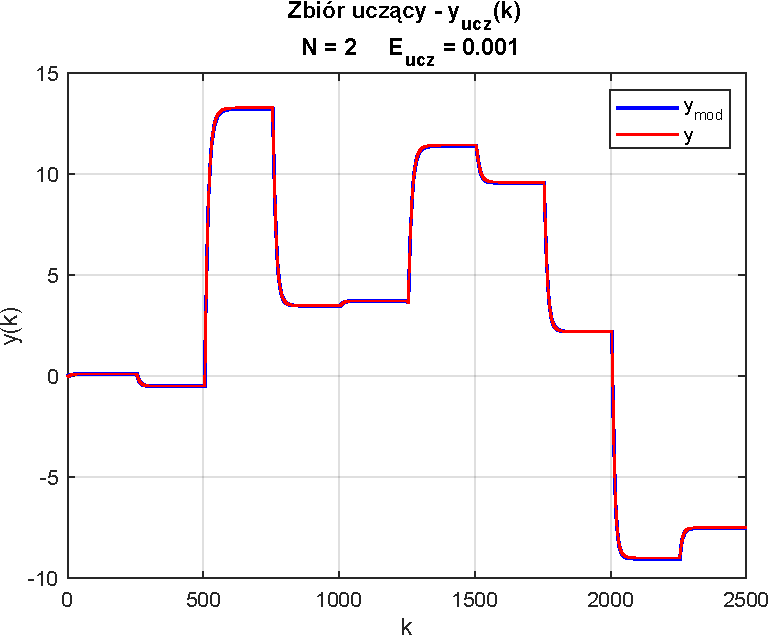
\includegraphics[width=0.45\textwidth]{pictures/arx_ucz_33}}
\hfill
\subfloat[Zbiór weryfikujący.]{
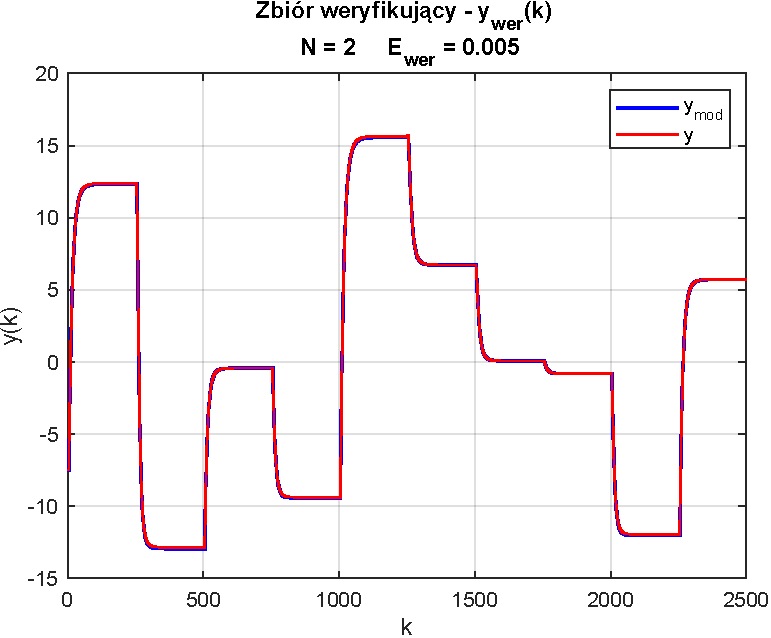
\includegraphics[width=0.45\textwidth]{pictures/arx_wer_33}}

\begin{center}
\Large \textbf{Model Wienera}
\end{center}

\subfloat[Zbiór uczący.]{
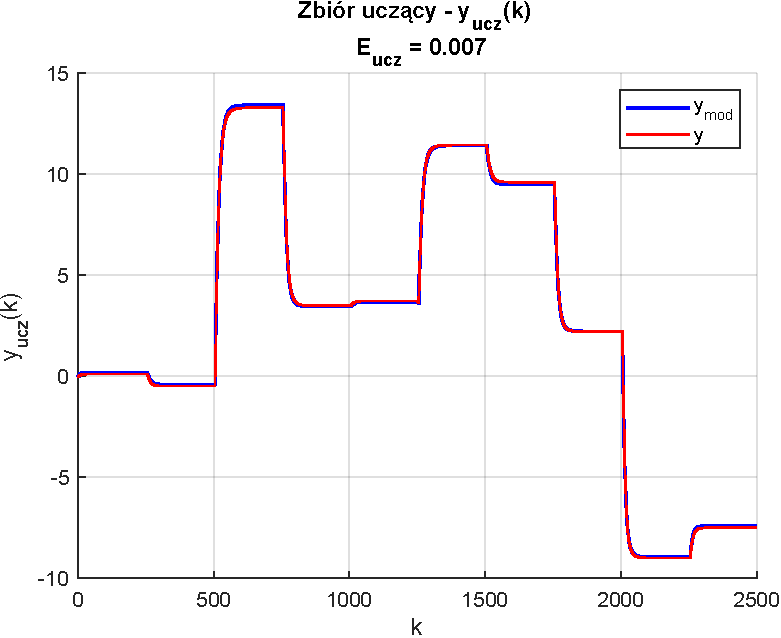
\includegraphics[width=0.45\textwidth]{pictures/arx_wien_ucz_33}}
\hfill
\subfloat[Zbiór weryfikujący.]{
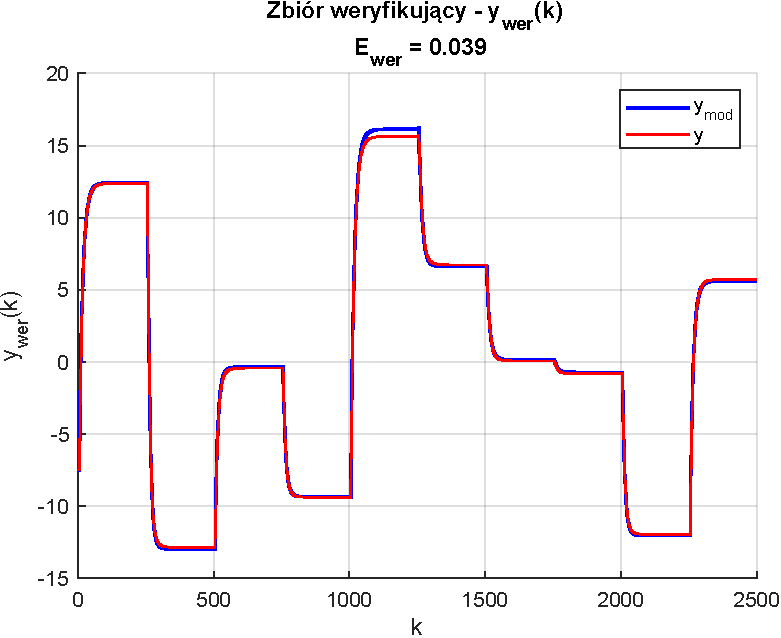
\includegraphics[width=0.45\textwidth]{pictures/arx_wien_wer_33}}
\caption{Porównanie przebiegu sygnału wyjściowego modelu dynamicznego i modelu Wienera w trybie bez rekurencji.}
\end{figure}

\newpage

\begin{figure}[h!]

\begin{center}
\Large \textbf{III sekwencja} \\
\vspace{0.5cm}
\Large \textbf{Model dynamiczny}
\end{center}

\centering
\subfloat[Zbiór uczący.]{
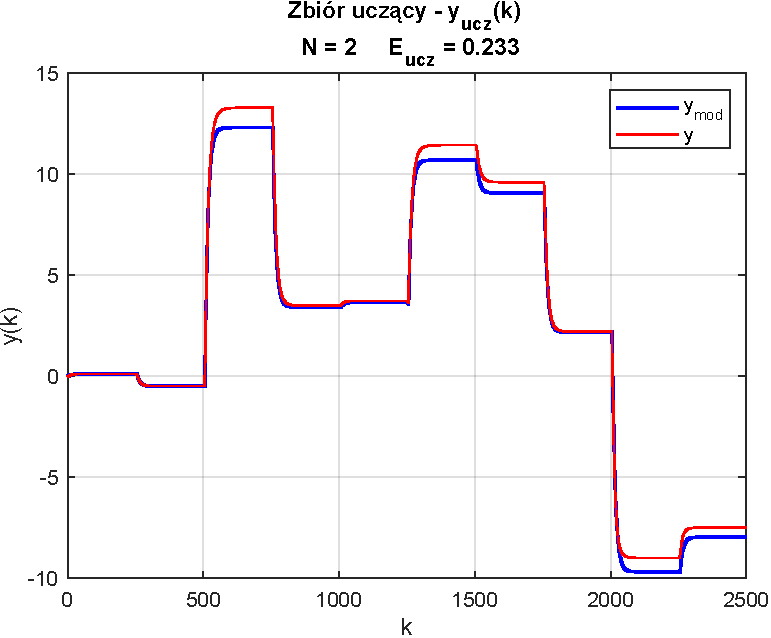
\includegraphics[width=0.45\textwidth]{pictures/oe_ucz_33}}
\hfill
\subfloat[Zbiór weryfikujący.]{
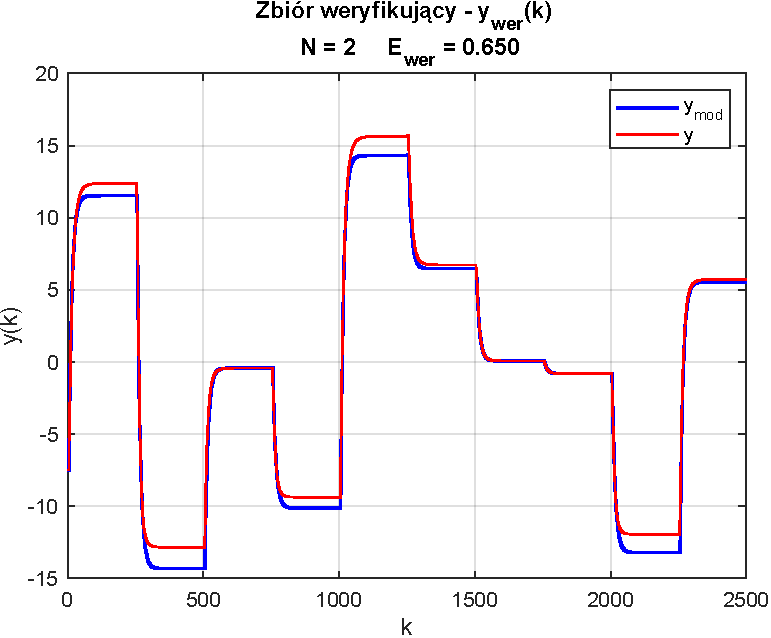
\includegraphics[width=0.45\textwidth]{pictures/oe_wer_33}}

\begin{center}
\Large \textbf{Model Wienera}
\end{center}

\subfloat[Zbiór uczący.]{
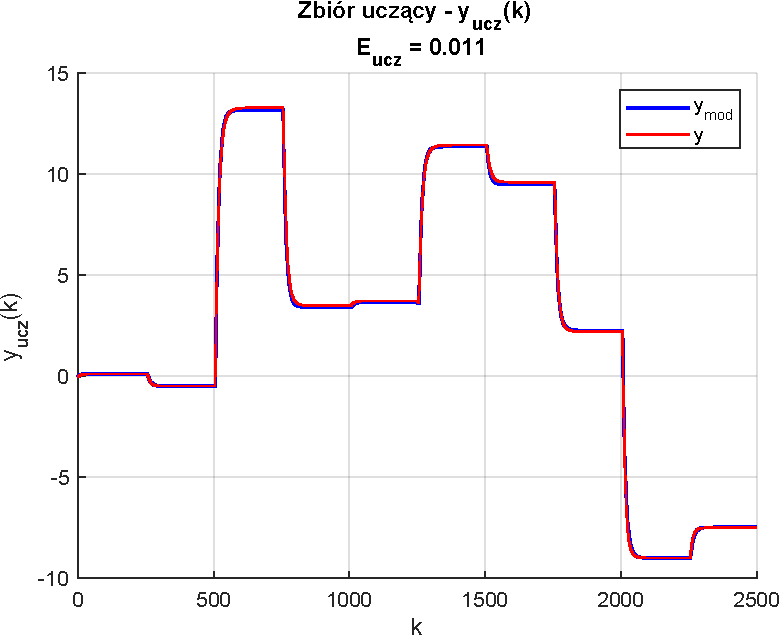
\includegraphics[width=0.45\textwidth]{pictures/oe_wien_ucz_33}}
\hfill
\subfloat[Zbiór weryfikujący.]{
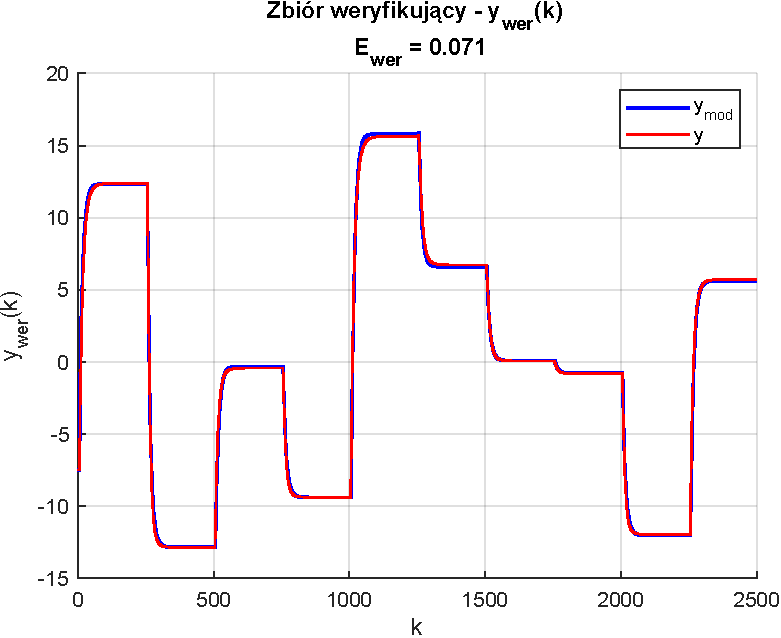
\includegraphics[width=0.45\textwidth]{pictures/oe_wien_wer_33}}
\caption{Porównanie przebiegu sygnału wyjściowego modelu dynamicznego i modelu Wienera w trybie rekurencyjnym.}
\end{figure}

Na podstawie powyższych wykresów, można wysnuć wniosek, że model Wienera został dobrze dostrojony, ponieważ w każdym z testowanych przypadków uzyskano błąd mniejszy niż przyjęty za graniczny $E = \num{0.1}$. Co ciekawe, strojąc model dobrano pewny współczynnik, który przemnażał wyjście liniowej dynamiki $v = f(u)$. Najlepszy rezultat uzyskano, gdy ta stała była równa wzmocnieniu statycznemu otrzymanej transmitancji, tj.

\begin{equation}
K_{stat} = \lim_{z \to 1} G(z)
\end{equation}

Wcześniej w równaniu różnicowymi zadbano, aby wzmocnienie statyczne wynosiło $1$, jednak mimo to, konieczne okazało się zastosowanie współczynnika regulującego. 

\newpage

\section{Następniki hiperboliczne}
W przypadku następników hiperbolicznych postąpiono analogicznie jak w przypadku modelu Hammersteina - zredukowano liczbę zbiorów przynależności jednocześnie starając się zachować dokładność osiągniętą dla następników liniowych. Z doświadczeń empirycznych postanowiono przyjąć taką samą postać następników jak poprzednio, tj.:

\begin{equation}
\text{Reguła n: Jeśli} \quad u^n(k) \quad \text{jest} \quad U_n, \quad \text{to}: \quad y^n(k) = a_n \cdot \sinh(b_n u^n(k) + c_n)
\end{equation}

Natomiast zbiory przynależności zmiennej $v$ prezentowały się następująco:

\begin{figure}[h!]
\centering
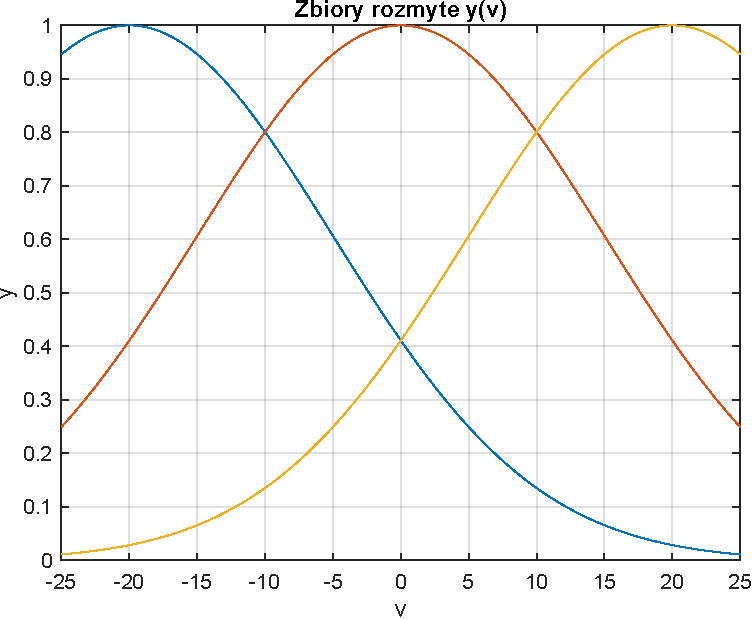
\includegraphics[width=0.6\textwidth]{pictures/fuzzy_set_wien_nlin}
\caption{Zbiory rozmyte - następniki hiperboliczne.}
\end{figure}

Z kolei dokładność aproksymacji charakterystyki statycznej przedstawiono na rys. \ref{static_char_wien_nlin}.

\begin{figure}[h!]
\centering
\subfloat[Zbiór uczący.]{
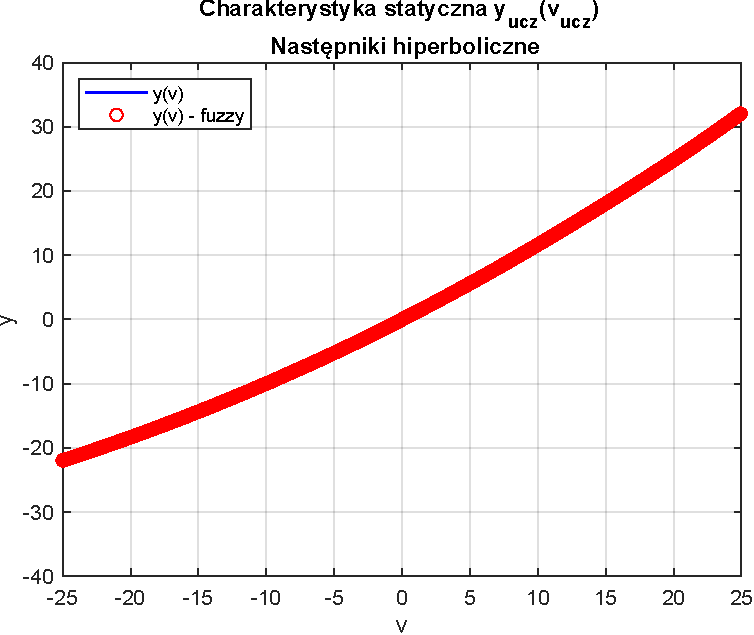
\includegraphics[width=0.45\textwidth]{pictures/static_char_wien_nlin_ucz}}
\hfill
\subfloat[Zbiór weryfikujący.]{
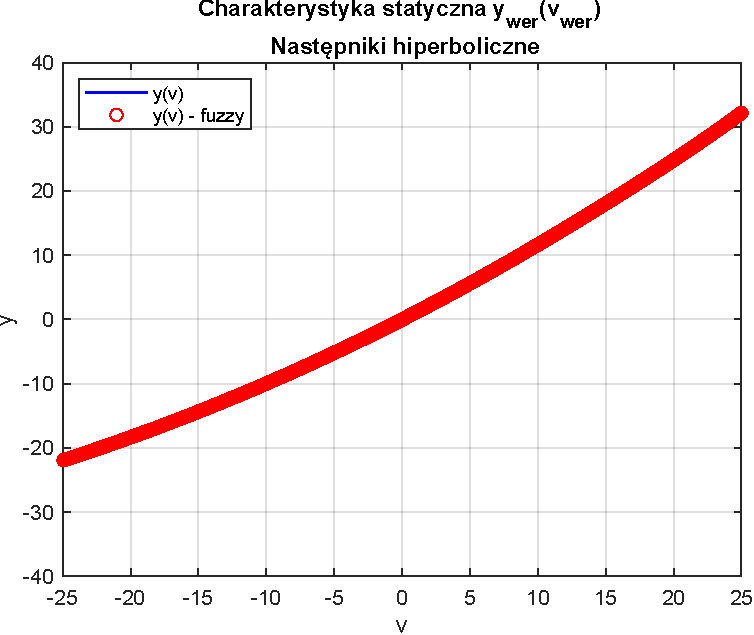
\includegraphics[width=0.45\textwidth]{pictures/static_char_wien_nlin_wer}}
\caption{Aproksymacja charakterystyki statycznej przez model rozmyty - następniki hiperboliczne.}
\label{static_char_wien_nlin}
\end{figure}

\newpage

Przystąpiono do testowania modeli, generując kolejne sekwencje sygnału sterującego.

%%%%%%%%%%%%%%%%%%%%%% PIERWSZA SEKWENCJA %%%%%%%%%%%%%%%%%%%%%%
\begin{figure}[h!]

\begin{center}
\Large \textbf{I sekwencja} \\
\vspace{0.5cm}
\Large \textbf{Model dynamiczny}
\end{center}

\centering
\subfloat[Zbiór uczący.]{
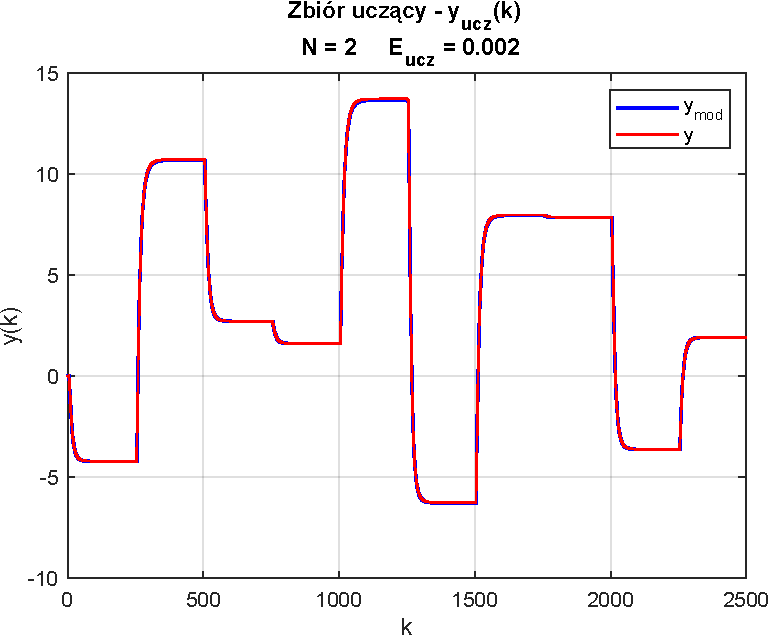
\includegraphics[width=0.45\textwidth]{pictures/arx_ucz_41}}
\hfill
\subfloat[Zbiór weryfikujący]{
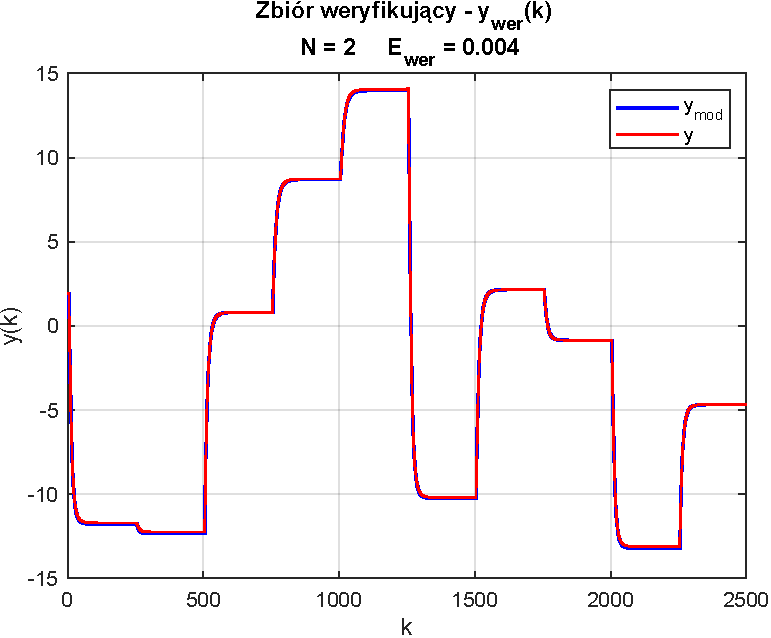
\includegraphics[width=0.45\textwidth]{pictures/arx_wer_41}}

\begin{center}
\Large \textbf{Model Wienera}
\end{center}

\subfloat[Zbiór uczący.]{
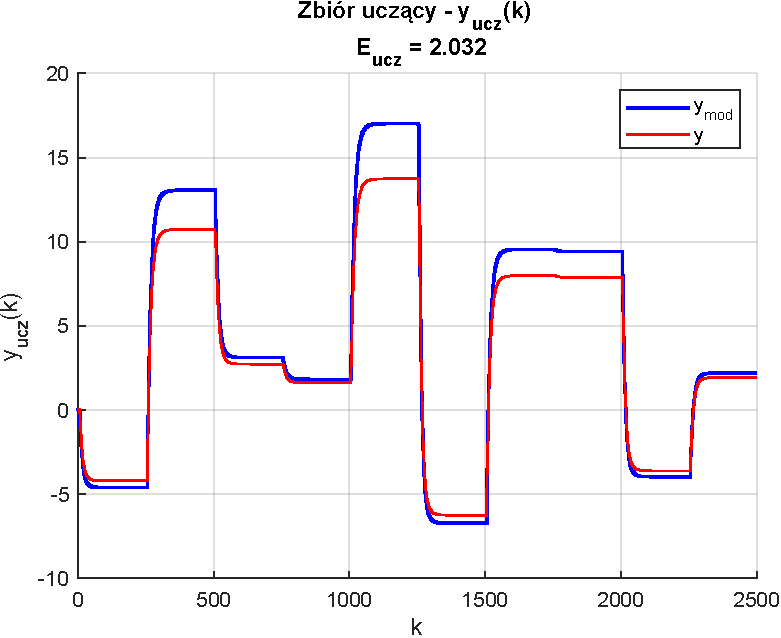
\includegraphics[width=0.45\textwidth]{pictures/arx_wien_ucz_41}}
\hfill
\subfloat[Zbiór weryfikujący]{
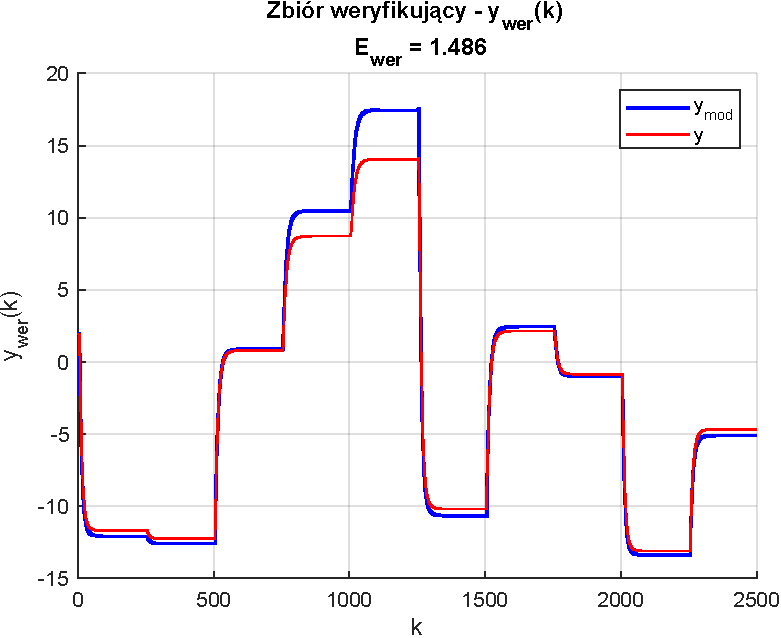
\includegraphics[width=0.45\textwidth]{pictures/arx_wien_wer_41}}
\caption{Porównanie przebiegu sygnału wyjściowego modelu dynamicznego i modelu Wienera w trybie bez rekurencji.}
\end{figure}

Po raz kolejny model Wienera wymagał ręcznego strojenia. Tym razem natomiast oprócz lokalnych poprawek modeli systemu rozmytego zdecydowano się na przemnożenie wyjścia modelu przez stałą. 

\newpage

\begin{figure}[h!]
\centering
\subfloat[Zbiór uczący.]{
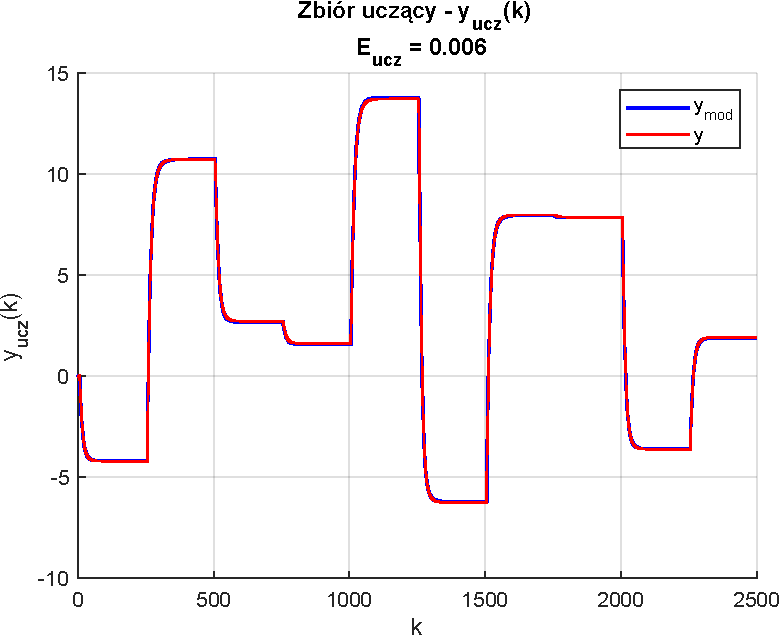
\includegraphics[width=0.7\textwidth]{pictures/arx_wien_ucz_42}}
\hfill
\subfloat[Zbiór weryfikujący]{
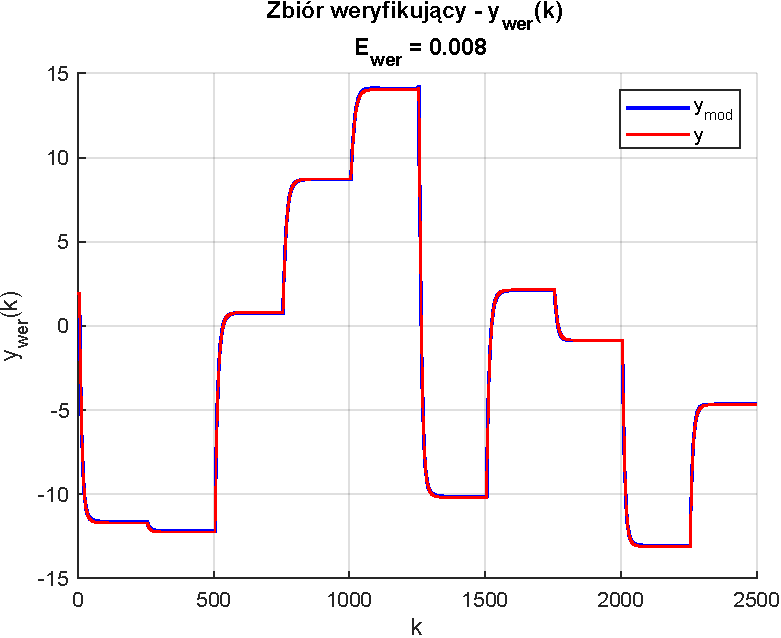
\includegraphics[width=0.7\textwidth]{pictures/arx_wien_wer_42}}
\caption{Przebiegi sygnału wyjściowego modelu Wienera w trybie bez rekurencji po dostrojeniu współczynników następników.}
\end{figure}

Udało się uzyskać satysfakcjonujące rezultaty. Model Wienera w trybie ARX po dostrojeniu prezentował się bardzo dobrze.

\newpage

\begin{figure}[h!]

\begin{center}
\Large \textbf{I sekwencja} \\
\vspace{0.5cm}
\Large \textbf{Model dynamiczny}
\end{center}

\centering
\subfloat[Zbiór uczący.]{
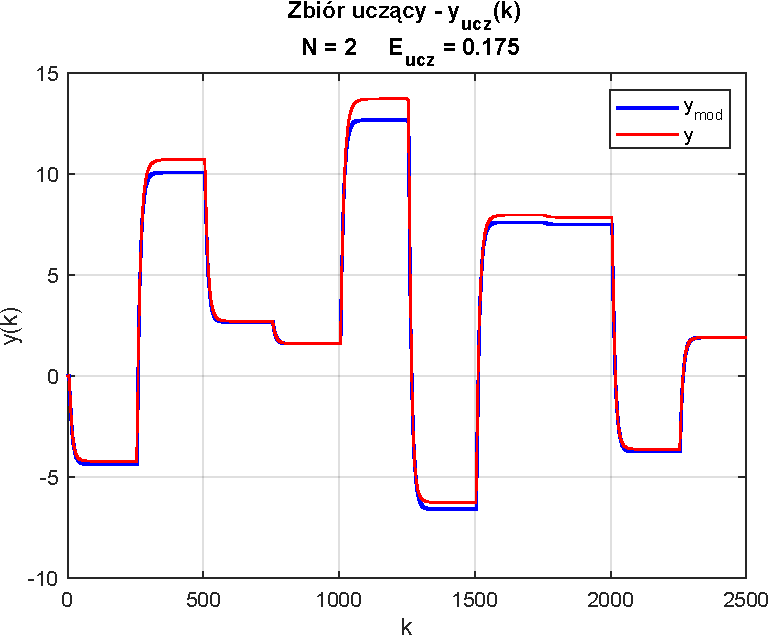
\includegraphics[width=0.45\textwidth]{pictures/oe_ucz_41}}
\hfill
\subfloat[Zbiór weryfikujący]{
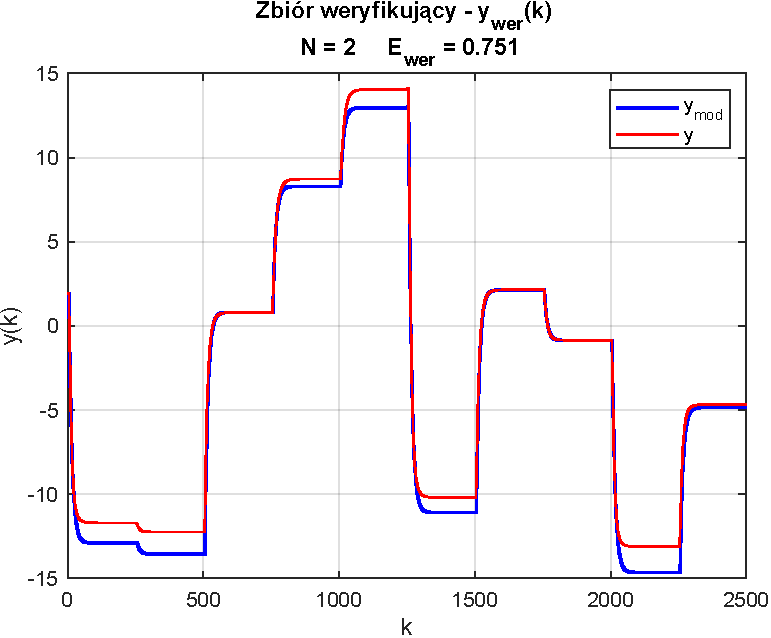
\includegraphics[width=0.45\textwidth]{pictures/oe_wer_41}}

\begin{center}
\Large \textbf{Model Wienera}
\end{center}

\subfloat[Zbiór uczący.]{
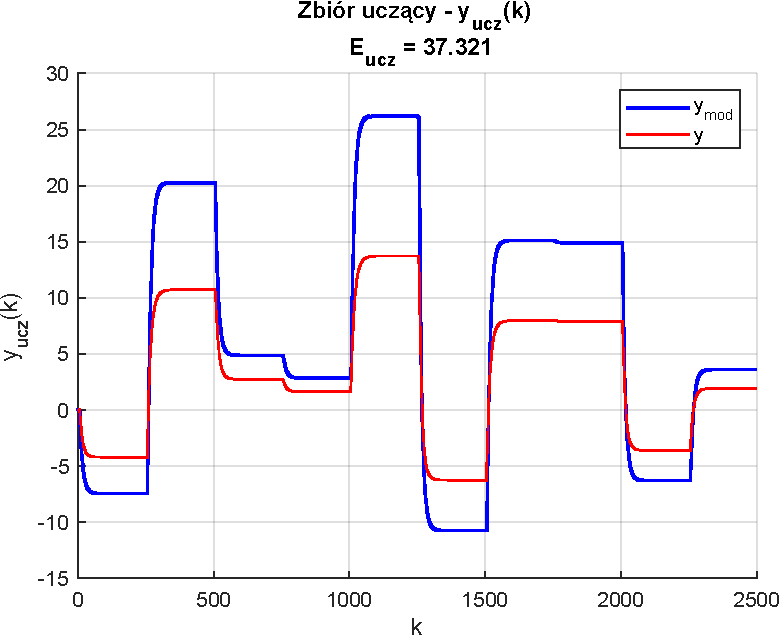
\includegraphics[width=0.45\textwidth]{pictures/oe_wien_ucz_41}}
\hfill
\subfloat[Zbiór weryfikujący]{
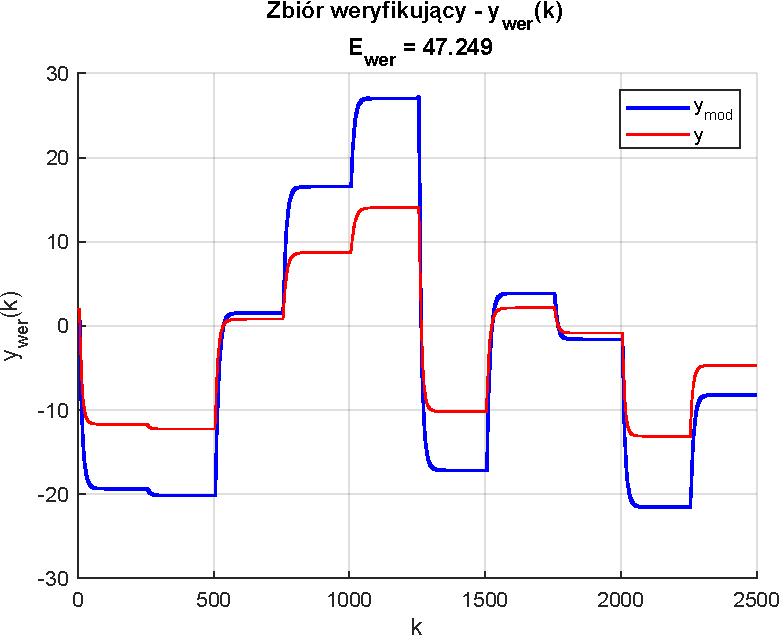
\includegraphics[width=0.45\textwidth]{pictures/oe_wien_wer_41}}
\caption{Porównanie przebiegu sygnału wyjściowego modelu dynamicznego i modelu Wienera w trybie rekurencyjnym.}
\end{figure}

Model testowany w trybie rekurencyjnym wymagał dużej ingerencji. Przede wszystkim przemnożenie wyjścia modelu przez stałą - w tym przypadku $\num{0.54}$ - znacznie poprawiło otrzymane wyniki. Dostrojenie modeli lokalnych pozwoliło uzyskać satysfakcjonujący rezultat.

\newpage

\begin{figure}[h!]
\centering
\subfloat[Zbiór uczący.]{
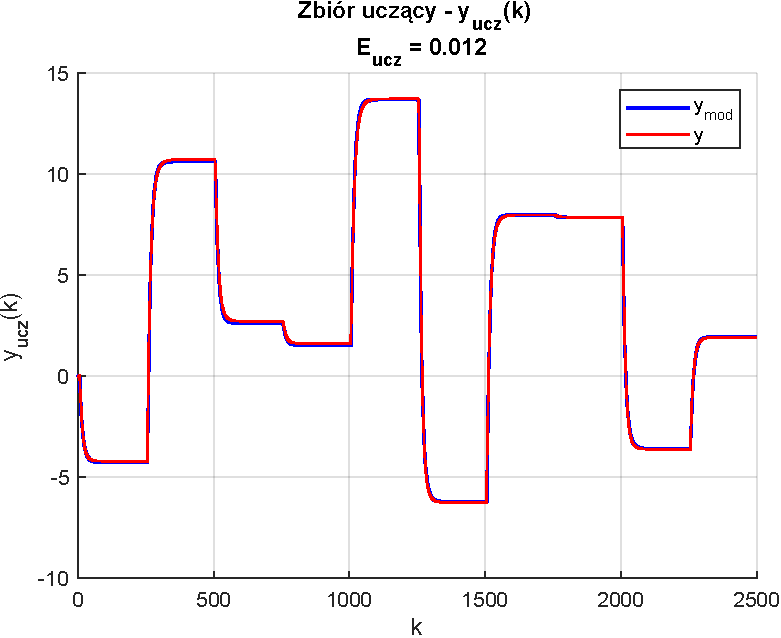
\includegraphics[width=0.7\textwidth]{pictures/oe_wien_ucz_42}}
\hfill
\subfloat[Zbiór weryfikujący]{
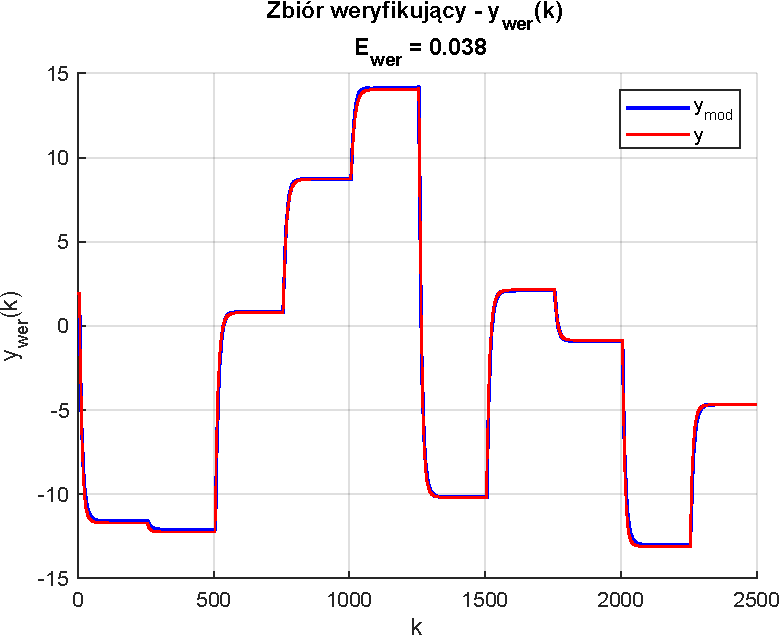
\includegraphics[width=0.7\textwidth]{pictures/oe_wien_wer_42}}
\caption{Przebiegi sygnału wyjściowego modelu Wienera w trybie rekurencyjnym po dostrojeniu współczynników następników.}
\end{figure}

Z tak wystrojony model rozmyty poddano kolejnym dwóm testom, generując odpowiednią sekwencję sygnału sterującego.

%%%%%%%%%%%%%%%%%%%%%% DRUGA SEKWENCJA %%%%%%%%%%%%%%%%%%%%%%
\begin{figure}[p!]

\begin{center}
\Large \textbf{II sekwencja} \\
\vspace{0.5cm}
\Large \textbf{Model dynamiczny}
\end{center}

\centering
\subfloat[Zbiór uczący.]{
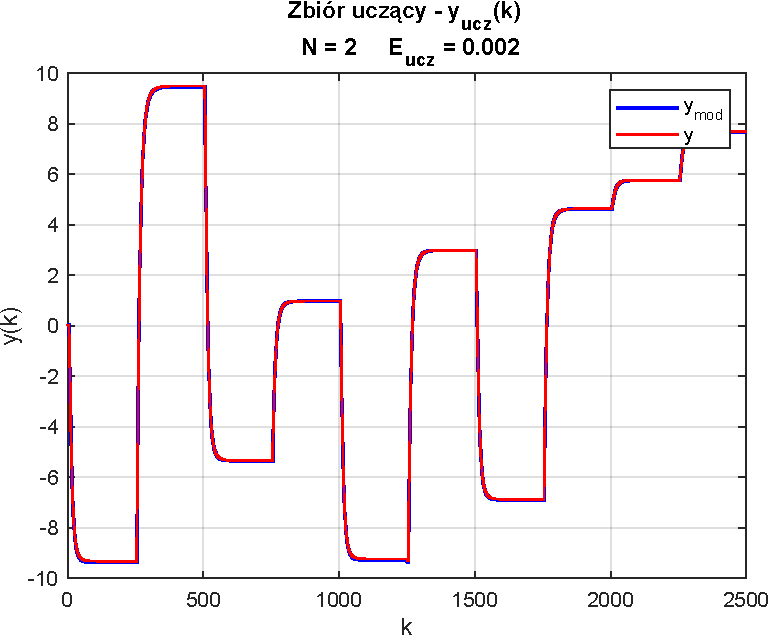
\includegraphics[width=0.45\textwidth]{pictures/arx_ucz_55}}
\hfill
\subfloat[Zbiór weryfikujący]{
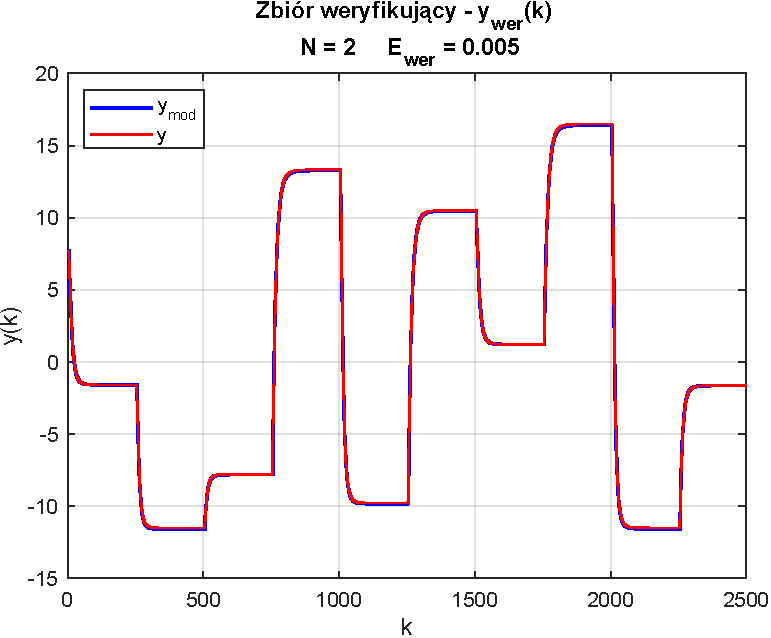
\includegraphics[width=0.45\textwidth]{pictures/arx_wer_55}}

\begin{center}
\Large \textbf{Model Wienera}
\end{center}

\subfloat[Zbiór uczący.]{
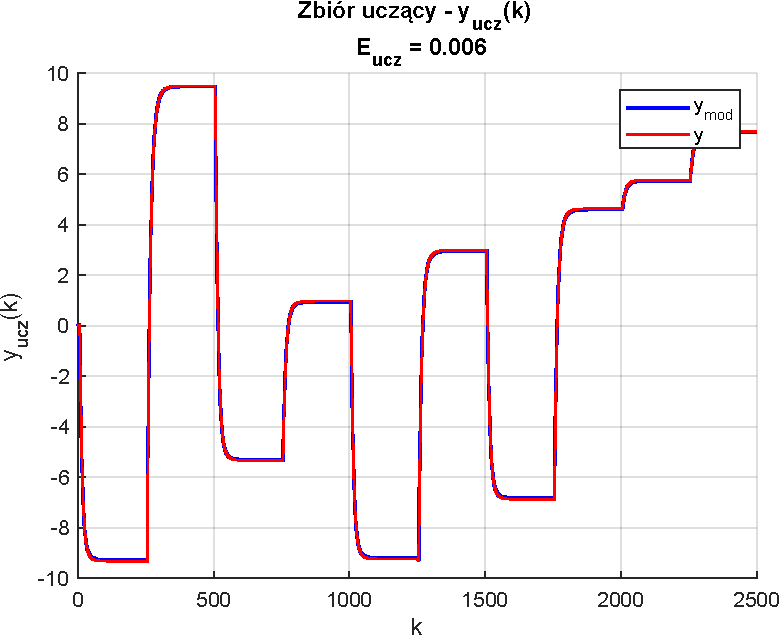
\includegraphics[width=0.45\textwidth]{pictures/arx_wien_ucz_55}}
\hfill
\subfloat[Zbiór weryfikujący]{
\includegraphics[width=0.45\textwidth]{pictures/arx_wien_wer_55}}
\caption{Porównanie przebiegu sygnału wyjściowego modelu dynamicznego i modelu Wienera w trybie bez rekurencji.}
\end{figure}

\begin{figure}[p!]

\begin{center}
\Large \textbf{II sekwencja} \\
\vspace{0.5cm}
\Large \textbf{Model dynamiczny}
\end{center}

\centering
\subfloat[Zbiór uczący.]{
\includegraphics[width=0.45\textwidth]{pictures/oe_ucz_55}}
\hfill
\subfloat[Zbiór weryfikujący]{
\includegraphics[width=0.45\textwidth]{pictures/oe_wer_55}}

\begin{center}
\Large \textbf{Model Wienera}
\end{center}

\subfloat[Zbiór uczący.]{
\includegraphics[width=0.45\textwidth]{pictures/oe_wien_ucz_55}}
\hfill
\subfloat[Zbiór weryfikujący]{
\includegraphics[width=0.45\textwidth]{pictures/oe_wien_wer_55}}
\caption{Porównanie przebiegu sygnału wyjściowego modelu dynamicznego i modelu Wienera w trybie rekurencyjnym.}
\end{figure}

%%%%%%%%%%%%%%%%%%%%%% TRZECIA SEKWENCJA %%%%%%%%%%%%%%%%%%%%%%
\begin{figure}[p!]

\begin{center}
\Large \textbf{III sekwencja} \\
\vspace{0.5cm}
\Large \textbf{Model dynamiczny}
\end{center}

\centering
\subfloat[Zbiór uczący.]{
\includegraphics[width=0.45\textwidth]{pictures/arx_ucz_66}}
\hfill
\subfloat[Zbiór weryfikujący]{
\includegraphics[width=0.45\textwidth]{pictures/arx_wer_66}}

\begin{center}
\Large \textbf{Model Wienera}
\end{center}

\subfloat[Zbiór uczący.]{
\includegraphics[width=0.45\textwidth]{pictures/arx_wien_ucz_66}}
\hfill
\subfloat[Zbiór weryfikujący]{
\includegraphics[width=0.45\textwidth]{pictures/arx_wien_wer_66}}
\caption{Porównanie przebiegu sygnału wyjściowego modelu dynamicznego i modelu Wienera w trybie bez rekurencji.}
\end{figure}

\newpage

\begin{figure}[h!]

\begin{center}
\Large \textbf{III sekwencja} \\
\vspace{0.5cm}
\Large \textbf{Model dynamiczny}
\end{center}

\centering
\subfloat[Zbiór uczący.]{
\includegraphics[width=0.45\textwidth]{pictures/oe_ucz_66}}
\hfill
\subfloat[Zbiór weryfikujący]{
\includegraphics[width=0.45\textwidth]{pictures/oe_wer_66}}

\begin{center}
\Large \textbf{Model Wienera}
\end{center}

\subfloat[Zbiór uczący.]{
\includegraphics[width=0.45\textwidth]{pictures/oe_wien_ucz_66}}
\hfill
\subfloat[Zbiór weryfikujący]{
\includegraphics[width=0.45\textwidth]{pictures/oe_wien_wer_66}}
\caption{Porównanie przebiegu sygnału wyjściowego modelu dynamicznego i modelu Wienera w trybie rekurencyjnym.}
\end{figure}

Na podstawie powyższych wykresów można wysnuć wniosek, że udało się osiągnąć zamierzony cel - zredukowano liczbę zbiorów rozmytych i tym samym modeli lokalnych przy zachowaniu wcześniej osiągniętej dokładności. Niemniej, ręczne dostrajanie współczynników następników hiperbolicznych było procesem czasochłonnym i mało intuicyjnym, bowiem chcąc poprawić działanie modelu w danym przedziale wartości często okazywało się, że należy zmienić parametry modelu, który w tym przedziale wydawał się być nieistotny. Ostateczny efekt uznano za satysfakcjonujący. 